\documentclass[11pt,oneside]{article}
\input{../../../Header/packages.sty}
\input{../../../Header/styleScript.sty}
\input{../../../Header/headerScript.sty}
\input{../../../Header/mathexpressions.sty}


\newcommand{\Skriptname}{Lektion: Die Flächenformel nach Heron}
\newcommand{\Autor}{Jonas Guler (Gu)}
\newcommand{\version}{\textit{v}1.0}

\begin{document}
\thispagestyle{plain}
\begin{center}
	{\Huge\textbf{Die Flächenformel nach Heron}}\\[3mm]
	{\large Abschluss der Satzgruppe des Pythagoras -- Flächeninhalt aus drei Seiten}\\[2mm]
	{\normalsize Name: \gap{6}\hspace{1cm} Datum: \gap{3}}
\end{center}
\vspace{2mm}
Bisher haben wir mit Pythagoras, Kathetensatz und Höhensatz nur in \textbf{rechtwinkligen} Dreiecken gerechnet. Heute zeigen wir: Mit diesen Werkzeugen lässt sich der Flächeninhalt \textbf{jedes} Dreiecks berechnen, wenn nur die drei Seiten $a$, $b$ und $c$ bekannt sind. Wir verwenden die üblichen Bezeichnungen: $a=\overline{BC}$, $b=\overline{CA}$, $c=\overline{AB}$, und $h_c$ ist die Höhe auf die Seite $c$ mit Fusspunkt $H_c$.
\begin{center}
	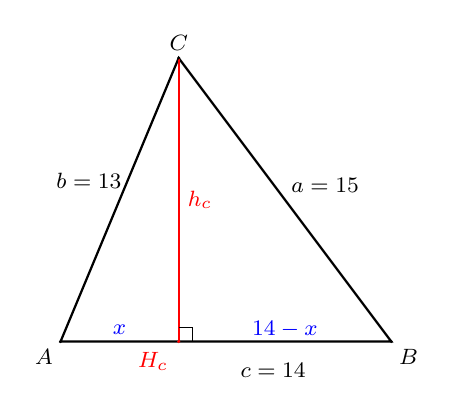
\begin{tikzpicture}[x=1cm, y=1cm, >=latex, font=\footnotesize, scale=0.6]
		\coordinate (A) at (0,0);
		\coordinate (B) at (7,0);
		\coordinate (C) at (2.5,6);
		\coordinate (H) at (2.5,0);
		\draw[line width=0.8pt] (A) -- (B) -- (C) -- cycle;
		\draw[color=red, line width=0.8pt] (C) -- (H);
		\draw (2.8,0) -- (2.8,0.3) -- (2.5,0.3);
		\begin{scriptsize}
			\fill (A) circle (1pt) node[below left] {$A$};
			\fill (B) circle (1pt) node[below right] {$B$};
			\fill (C) circle (1pt) node[above] {$C$};
			\fill[red] (H) circle (1pt) node[below left=1pt, red] {$H_c$};
			\draw (0.6,3.4) node {$b=13$};
			\draw (5.6,3.3) node {$a=15$};
			\draw[color=red] (2.95,3) node {$h_c$};
			\draw[color=blue] (1.25,0.25) node {$x$};
			\draw[color=blue] (4.75,0.25) node {$14-x$};
			\draw (4.5,-0.6) node {$c=14$};
		\end{scriptsize}
	\end{tikzpicture}
\end{center}

%############################################################################################
\section{Einstieg: Fläche aus drei Seiten}
\begin{aufgabe}[Entdeckungsaufgabe, Partnerarbeit] % Idee: Geometrie 1 Aufgaben (Niederberger) Kap. 5, Nr. 81 a) und d)
	\textbf{Teil A: Ein Dreieck ohne rechten Winkel.} Gegeben ist das Dreieck $\triangle ABC$ in der Figur oben mit $a=15$ cm, $b=13$ cm und $c=14$ cm. Die Höhe $h_c$ zerlegt das Dreieck in zwei \textbf{rechtwinklige} Teildreiecke.
	\begin{enumerate}[label=\alph*)]
		\item Stelle in beiden Teildreiecken den Satz des Pythagoras für $h_c^2$ auf.
		\item Setze die beiden Terme gleich und berechne $x$. \textit{Tipp: Die Terme $x^2$ fallen weg.}
		\item Berechne $h_c$ und den Flächeninhalt $A$ des Dreiecks.
	\end{enumerate}
	\karos{5}
	\tcbbreak
	\textbf{Teil B: Derselbe Weg mit Variablen.} Jetzt soll das Dreieck ganz allgemein die Seiten $a$, $b$, $c$ haben. Wir gehen genau gleich vor wie in Teil A und erhalten so eine Formel, die den Flächeninhalt \textbf{nur aus den drei Seiten} berechnet.
	\begin{enumerate}[label=\alph*), resume]
		\item \textbf{Zweimal Pythagoras:} Ergänze für die beiden Teildreiecke
		\[h_c^2=\gap{3}\qquad\text{und}\qquad h_c^2=\gap{3}.\]
		Setze gleich und zeige, dass $x=\dfrac{b^2+c^2-a^2}{2c}$ gilt.
	\end{enumerate}
	\karos{2}
	\begin{enumerate}[label=\alph*), resume]
		\item \textbf{Die Höhe:} Im linken Teildreieck gilt $h_c^2=b^2-x^2=(b+x)(b-x)$ (3.\ binomische Formel). Setze $x$ ein und bringe auf einen Bruchstrich:
		\[b+x=\frac{2bc+b^2+c^2-a^2}{2c}=\frac{(\gap{1.2})^2-a^2}{2c},\qquad b-x=\frac{2bc-b^2-c^2+a^2}{2c}=\frac{a^2-(\gap{1.2})^2}{2c}.\]
		\item \textbf{Nochmals die 3.\ binomische Formel:} Zerlege beide Zähler in ein Produkt:
		\[(b+c)^2-a^2=(\gap{2})(\gap{2}),\qquad a^2-(b-c)^2=(\gap{2})(\gap{2}).\]
		\item \textbf{Die Fläche:} Wegen $A=\frac12\,c\,h_c$ ist $A^2=\frac14\,c^2\,h_c^2=\frac14\,c^2\,(b+x)(b-x)$. Setze ein und kürze. Ergänze:
		\[A^2=\frac{(a+b+c)\cdot(\gap{1.8})\cdot(\gap{1.8})\cdot(\gap{1.8})}{16}.\]
	\end{enumerate}
	\karos{2}
	\begin{enumerate}[label=\alph*), resume]
		\item \textbf{Schöner schreiben:} Mit dem \textbf{halben Umfang} $s=\frac{a+b+c}{2}$ gilt $a+b+c=2s$. Zeige, dass $b+c-a=2(s-a)$ ist, und ergänze die beiden anderen Faktoren:
		\[a-b+c=\gap{2},\qquad a+b-c=\gap{2}.\]
		Setze in g) ein und vereinfache so weit wie möglich:
		\[A^2=\gap{5}\qquad\Longrightarrow\qquad A=\gap{5}\]
		\item \textbf{Kontrolle:} Teste deine Formel am Dreieck aus Teil A und am rechtwinkligen Dreieck mit $a=3$, $b=4$, $c=5$.
	\end{enumerate}
	\karos{1.5}
\end{aufgabe}

\newpage
%############################################################################################
\section{Die Formel von Heron}
Die Formel aus Aufgabe 1.1 gilt für \textbf{jedes} Dreieck. Sie wird nach \textbf{Heron von Alexandria} (ca.\ 10--75 n.\,Chr.) benannt, der sie in seinem Werk \textit{Metrica} bewiesen hat.
\begin{satz}[Flächenformel nach Heron]
	Ein Dreieck habe die Seitenlängen $a$, $b$, $c$ und den halben Umfang $s=\dfrac{a+b+c}{2}$. Dann gilt für seinen Flächeninhalt
	\[A=\sqrt{s\cdot(s-a)\cdot(s-b)\cdot(s-c)}.\]
\end{satz}
\begin{beweis}[Zusammenfassung]
	Den Beweis hast du in Aufgabe 1.1, Teil B, selbst geführt. Die vier Schritte:
	\begin{enumerate}[label=(\arabic*)]
		\item \textbf{Zweimal Pythagoras} in den Teildreiecken liefert $x=\dfrac{b^2+c^2-a^2}{2c}$.
		\item $h_c^2=(b+x)(b-x)$ und \textbf{zweimal die 3.\ binomische Formel} ergeben \[h_c^2=\frac{(a+b+c)(b+c-a)(a-b+c)(a+b-c)}{4c^2}.\]
		\item Aus $A^2=\frac14\,c^2\,h_c^2$ kürzt sich $c^2$ weg.
		\item Jeder Faktor ist das Doppelte von $s$, $s-a$, $s-b$ bzw.\ $s-c$: $A^2=\dfrac{16\,s(s-a)(s-b)(s-c)}{16}$.
	\end{enumerate}
\end{beweis}
\textbf{Bemerkungen:}
\begin{itemize}
	\item \textbf{Kernbotschaft:} Drei Seiten legen ein Dreieck fest (Kongruenzsatz SSS), also auch seinen Flächeninhalt. Heron liefert ihn \textbf{direkt}, ohne dass man eine Höhe kennen muss.
	\item Die Formel ist \textbf{symmetrisch} in $a$, $b$, $c$: Es spielt keine Rolle, welche Seite wie heisst. Sie gilt für spitz-, recht- und stumpfwinklige Dreiecke.
	\item \textbf{Vorgehen:} Zuerst $s$ berechnen, dann $s-a$, $s-b$, $s-c$ (Kontrolle: $(s-a)+(s-b)+(s-c)=s$), erst am Schluss die Wurzel ziehen.
	\item Kennt man $A$, so erhält man jede Höhe aus $A=\frac12\,a\,h_a$, also $h_a=\dfrac{2A}{a}$ (analog $h_b$ und $h_c$).
	\item Die Satzgruppe des Pythagoras ist der Werkzeugkasten für den Beweis: Heron ist \textit{zweimal Pythagoras plus Algebra}.
\end{itemize}

\begin{beispiel}
	Ein Dreieck hat die Seiten $a=7$ cm, $b=8$ cm und $c=9$ cm. Berechne den Flächeninhalt $A$ und die Höhe $h_c$.
\end{beispiel}
\karos{4.5}

%############################################################################################
\section{Übungen}
\setcounter{aufg}{0}
\begin{aufgabe}[Grundaufgaben] % angelehnt an Geometrie 1 Aufgaben Kap. 5, Nr. 81 a)
	Berechne den Flächeninhalt der Dreiecke mit den gegebenen Seitenlängen (in cm). Kontrolliere bei den rechtwinkligen Dreiecken mit $\frac{a\cdot b}{2}$ und beim gleichschenkligen Dreieck über die Höhe auf die Basis.
	\begin{enumcols}[3]
		\item $5,\ 12,\ 13$
		\item $10,\ 10,\ 12$
		\item $4,\ 5,\ 6$
		\item $6,\ 7,\ 8$
		\item $2.5,\ 6,\ 6.5$
		\item $9,\ 10,\ 17$
	\end{enumcols}
	\karos{9}
\end{aufgabe}

\begin{aufgabe}[Alle drei Höhen]
	Ein Dreieck hat die Seiten $a=25$ cm, $b=39$ cm und $c=56$ cm.
	\begin{enumerate}[label=\alph*)]
		\item Berechne den Flächeninhalt mit der Formel von Heron.
		\item Berechne alle drei Höhen $h_a$, $h_b$ und $h_c$. Welche ist am längsten? Begründe ohne Rechnung, weshalb das so sein muss.
	\end{enumerate}
	\karos{5}
\end{aufgabe}

\begin{aufgabe}[Das gleichseitige Dreieck] % Idee: Geometrie 1 Aufgaben Kap. 5, Nr. 81 a)
	Im Skript haben wir mit Pythagoras die Höhe eines gleichseitigen Dreiecks mit Seitenlänge $a$ berechnet.
	\begin{enumerate}[label=\alph*)]
		\item Leite mit der Formel von Heron eine Formel für den Flächeninhalt eines gleichseitigen Dreiecks mit Seitenlänge $a$ her.
		\item Kontrolliere dein Resultat mit der bekannten Höhe $h=\frac{a}{2}\sqrt3$.
	\end{enumerate}
	\karos{5}
\end{aufgabe}

\begin{aufgabe}[Das Grundstück]
	\begin{minipage}{0.55\linewidth}
		Ein Grundstück $ABCD$ hat die Form eines Vierecks. Ein Geometer hat die vier Seiten und die Diagonale $\overline{AC}$ gemessen:\\[2mm]
		$\overline{AB}=40$ m, $\overline{BC}=25$ m, $\overline{CD}=30$ m,\\ $\overline{DA}=35$ m, $\overline{AC}=45$ m.\\[2mm]
		Berechne die Fläche des Grundstücks. Das Land kostet $850$ Fr.\ pro m$^2$. Wie teuer ist das Grundstück?
	\end{minipage}
	\hfill
	\begin{minipage}{0.4\linewidth}
		\centering
		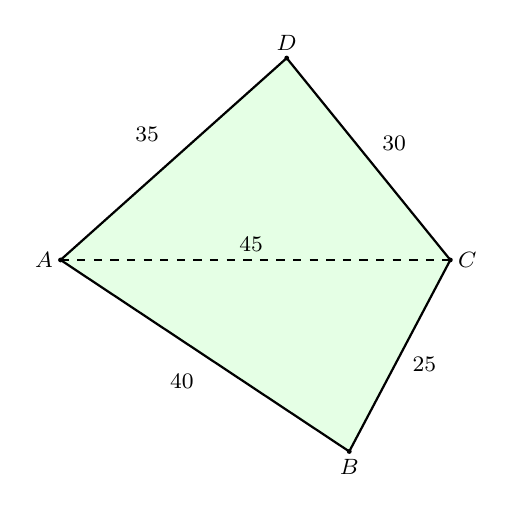
\begin{tikzpicture}[x=1cm, y=1cm, font=\footnotesize, scale=0.11]
			\coordinate (A) at (0,0);
			\coordinate (B) at (33.33,-22.11);
			\coordinate (C) at (45,0);
			\coordinate (D) at (26.11,23.31);
			\filldraw[fill=green!10, line width=0.8pt] (A) -- (B) -- (C) -- (D) -- cycle;
			\draw[dashed] (A) -- (C);
			\begin{scriptsize}
				\fill (A) circle (8pt) node[left] {$A$};
				\fill (B) circle (8pt) node[below] {$B$};
				\fill (C) circle (8pt) node[right] {$C$};
				\fill (D) circle (8pt) node[above] {$D$};
				\draw (14,-14) node {$40$};
				\draw (42,-12) node {$25$};
				\draw (38.5,13.5) node {$30$};
				\draw (10,14.5) node {$35$};
				\draw (22,1.8) node {$45$};
			\end{scriptsize}
		\end{tikzpicture}
	\end{minipage}
	\par\karos{5}
\end{aufgabe}

\begin{aufgabe}[Wenn die Formel streikt] % Idee: Dreiecksungleichung
	Wende die Formel von Heron auf die folgenden Seitenlängen (in cm) an. Was stellst du fest? Versuche jeweils, das Dreieck zu konstruieren, und erkläre, was geometrisch los ist.
	\begin{enumcols}[2]
		\item $3,\ 4,\ 7$
		\item $2,\ 3,\ 6$
	\end{enumcols}
	Für welche Seitenlängen $a$, $b$, $c$ liefert die Formel also überhaupt einen Flächeninhalt?\par
	\karos{5}
\end{aufgabe}

\begin{aufgabe}[$\bigstar$ Knobelaufgabe: Heron-Dreiecke]
	Dreiecke mit ganzzahligen Seiten \textbf{und} ganzzahligem Flächeninhalt heissen \textbf{Heron-Dreiecke}. Das Dreieck aus der Einstiegsaufgabe ($13$, $14$, $15$) ist ein solches.
	\begin{enumerate}[label=\alph*)]
		\item Das Dreieck $13$, $14$, $15$ lässt sich aus zwei rechtwinkligen Dreiecken mit ganzzahligen Seiten zusammensetzen. Welche sind es? \textit{Tipp: Schau dir die Werte von $x$ und $h_c$ aus Teil A an.}
		\item Lege die rechtwinkligen Dreiecke $5$, $12$, $13$ und $12$, $16$, $20$ entlang der gemeinsamen Kathete $12$ aneinander. Welche Seitenlängen hat das neue Dreieck? Berechne seinen Flächeninhalt auf zwei Arten: über die Teildreiecke und mit Heron.
		\item Finde selbst ein weiteres Heron-Dreieck, das nicht rechtwinklig ist.
	\end{enumerate}
	\karos{7}
\end{aufgabe}

\begin{aufgabe}[$\bigstar$ Zusatz: Der Inkreis]
	Der Inkreis eines Dreiecks hat den Mittelpunkt $I$ und den Radius $r$.
	\begin{enumerate}[label=\alph*)]
		\item Zerlege das Dreieck in die drei Teildreiecke $\triangle ABI$, $\triangle BCI$ und $\triangle CAI$ und zeige: $A=r\cdot s$.
		\item Berechne den Inkreisradius des Dreiecks mit $a=15$, $b=13$, $c=14$ aus der Einstiegsaufgabe.
	\end{enumerate}
	\karos{5}
\end{aufgabe}

\end{document}
